\documentclass[runningheads]{llncs}

% ---------------------------------------------------------------
% Include basic ECCV package
 
% TODO REVIEW: Insert your submission number below by replacing '*****'
% TODO FINAL: Comment out the following line for the camera-ready version
% \usepackage[review,year=2024,ID=4970]{eccv}
% TODO FINAL: Un-comment the following line for the camera-ready version
\usepackage{eccv}

% OPTIONAL: Un-comment the following line for a version which is easier to read
% on small portrait-orientation screens (e.g., mobile phones, or beside other windows)
%\usepackage[mobile]{eccv}


% ---------------------------------------------------------------
% Other packages

% Commonly used abbreviations (\eg, \ie, \etc, \cf, \etal, etc.)

\usepackage{xcolor}  
\usepackage{booktabs,tabularx,caption}
\usepackage{multirow}
\usepackage{soul}
\usepackage{comment}
\usepackage{mathrsfs}
\usepackage{textcomp}
\usepackage{bbm}
\usepackage{verbatim}
\usepackage[accsupp]{axessibility}
\usepackage{wrapfig}
\usepackage{times}
\usepackage{epsfig}
\usepackage{graphicx}
% \usepackage{subfig}
\usepackage{eccvabbrv}
\usepackage[export]{adjustbox}
% Include other packages here, before hyperref.
\usepackage{graphicx}
\usepackage{booktabs}
\usepackage{float}

% The "axessiblity" package can be found at: https://ctan.org/pkg/axessibility?lang=en
\usepackage[accsupp]{axessibility}  % Improves PDF readability for those with disabilities.
%\usepackage{color}
\definecolor{green}{rgb}{0, 0.5, 0}
\definecolor{orange}{rgb}{0.8, 0.6, 0.2}
\definecolor{red}{rgb}{1.0, 0.0, 0.0}
\definecolor{teal}{rgb}{0.0, 0.4, 0.4}
\definecolor{purple}{rgb}{0.65,0,0.65}
\definecolor{saffron}{rgb}{0.95,0.75,0.2}
\definecolor{turquoise}{rgb}{0.0,0.5,0.5}
\definecolor{black}{rgb}{0.0, 0.0, 0.0}
\definecolor{gray}{rgb}{0.5, 0.5, 0.5}
\definecolor{blue}{rgb}{0.0, 0.0, 1.0}

\newcommand{\fg}[1]{{\color{orange}#1}}
\newcommand{\fgc}[1]{{\color{gray}[FG: #1]}}

\newcommand{\rqw}[1]{{\color{black}#1}}
\newcommand{\rqc}[1]{{\color{teal}[RQ: #1]}}

\newcommand{\agp}[1]{{\color{black}#1}}
\newcommand{\rz}[1]{{\color{black}#1}}
\newcommand{\rzz}[1]{{\color{black}#1}}
\newcommand{\chk}[1]{{\color{black}#1}}

\newcommand{\xeable}{{\color{black}moveable~}}
\newcommand{\Xeable}{{\color{black}Moveable~}}


% ---------------------------------------------------------------
% Hyperref package

% It is strongly recommended to use hyperref, especially for the review version.
% Please disable hyperref *only* if you encounter grave issues.
% hyperref with option pagebackref eases the reviewers' job, but should be disabled for the final version.
%
% If you comment hyperref and then uncomment it, you should delete
% main.aux before re-running LaTeX.
% (Or just hit 'q' on the first LaTeX run, let it finish, and you
%  should be clear).

% TODO FINAL: Comment out the following line for the camera-ready version
% \usepackage[pagebackref,breaklinks,colorlinks,citecolor=eccvblue]{hyperref}
% TODO FINAL: Un-comment the following line for the camera-ready version
\usepackage{hyperref}

% Support for ORCID icon
\usepackage{orcidlink}


\begin{document}

% ---------------------------------------------------------------
% TODO REVIEW: Replace with your title
\title{Active Coarse-to-Fine Segmentation of Moveable Parts from Real Images} 

% TODO REVIEW: If the paper title is too long for the running head, you can set
% an abbreviated paper title here. If not, comment out.
% \titlerunning{Abbreviated paper title}

% TODO FINAL: Replace with your author list. 
% Include the authors' OCRID for the camera-ready version, if at all possible.
\author{Ruiqi Wang\inst{1}\orcidlink{0009-0000-3379-6103} \and
Akshay Gadi Patil\inst{1}\orcidlink{0000-0003-1429-3804} \and
Fenggen Yu\inst{1}\orcidlink{0000-0003-1591-4668}\and
Hao Zhang\inst{1,2}\orcidlink{0000-0003-1991-119X}}

% TODO FINAL: Replace with an abbreviated list of authors.
\authorrunning{Ruiqi Wang et al.}
% First names are abbreviated in the running head.
% If there are more than two authors, 'et al.' is used.

% TODO FINAL: Replace with your institution list.
\institute{Simon Fraser University, Burnaby, Canada\\
\email{\{ruiqi\_w,agadipat,fenggen\_yu,haoz\}@sfu.ca} 
\and 
Amazon
\vspace{-10pt}}

\maketitle

\begin{center}
     \centering
     % \captionsetup{type=figure}
     \includegraphics[width=\textwidth]{figs/teaser.pdf}
     \vspace{-10pt}
     \captionof{figure}{\rzz{Our} instance segmentation of \xeable parts, with semantic labels, on real-world photos. Comparison is made with OPDFormer-C \rzz{(OPD = {\em openable\/} part detection)}, the current state of the art, where small red \textcolor{red}{\textbf{$\times$}}s indicate \rz{erroneous or missed labels.} \chk{Our method generalizes to {\em non-openable\/} parts, e.g., on lamps and bottles (top right).}
     As an application of accurate \xeable part segmentation, we can manipulate 3D reconstructions of articulated objects (bottom right). } % and more details in Section~\ref{sec:app}.}
     \label{fig:teaser}
\end{center}%
 \begin{abstract}
The current study investigated possible human-robot kinaesthetic interaction using a variational recurrent neural network model, called PV-RNN, which is based on the free energy principle.
Our prior robotic studies using PV-RNN showed that the nature of interactions between top-down expectation and bottom-up inference is strongly affected by a parameter, called the meta-prior, which regulates the complexity term in free energy.
% The current study examines how the behaviours of robots alter by changing the meta-prior $w$ in human-robot kinaesthetic interaction.
The current study examines how changing the meta-prior $w$ in the interaction phase affects the counter force generated when an experimenter attempts to induce movement pattern transitions familiar to the robot through its prior training.
The study also compares the counter force generated when trained transitions are induced by a human experimenter and when untrained transitions are induced.
Our experimental results indicated that (1) the human experimenter needs more/less force to induce trained transitions when $w$ is set with larger/smaller values, (2) the human experimenter needs more force to act on the robot when he attempts to induce untrained as opposed to trained movement pattern transitions.
Our analysis of time development of essential variables and values in PV-RNN during bodily interaction clarified the mechanism by which gaps in actional intentions between the human experimenter and the robot can be manifested as reaction forces between them.


%% Hiroki writing 2022-11-4
%Current study investigates the dynamics of the latent states during human-robot kinaesthetic interaction using PV-RNN.
%We have achieved to observe and analyse the internal state of an RNN model based on the free energy principle, during real-time human-robot interaction.
%Essential characteristics observed in the previous study of this variational recurrent neural network model, PV-RNN, is that by changing a meta prior $w$, the balance between the top-down intention and the bottom-up perceptual reality changes.
%In the current study, we examined how changing the weighting parameter $w$ between accuracy and complexity in free energy principle affects the humanoid robot's behaviour through human-robot interaction. We have conducted some human-robot kinaesthetic interaction experiments with various $w$ and quantitatively analysed the latent variable and the force applied to the humanoid robot. We have observed that the force required to change the robot's intention has increased, both when the top-down intention was strengthened by changing the $w$ and when corresponding switch of its primitive was against the experience of the RNN during its training. The study confirms through quantitative analysis that by increasing or decreasing the $w$ in PV-RNN, humanoid robot leads or follows the human counterpart during the human-robot kinaesthetic interaction.

\begin{comment}
Comment from Jun #2
・最後にQualitativeな結果(インパクト)が欲しい
・Current study investigates the problem on~と書き出すのが一般的
・最初の一文と最後の一文を対応させる
・最後の一文はもう少しAbstractかつ包括的に
\end{comment}

\begin{comment}
Comment from Jun #1
We investigated how the kinaesthetic human-robot interaction can affect the internal state of a model based on the free energy principle. 
=> how the internal state is affected is not the most important point in this study. This part should be rewritten.

The key function of this variational recurrent neural network model, PV-RNN, is that by changing a meta prior $w$, it takes a balance between the "complexity” term and the ”accuracy” term which corresponds to a top-down intention and a bottom-up perceptual reality in the free energy principle, respectively. 
=> This is not key function of PV-RNN. It is an essential characteristics observed in the previous study. The grammar after $w$ is something strange. Rewrite these.

This research has conducted a human-robot interaction experiment with a robotic agent in a kinaesthetic sense.
=> The sentence is not good. "in a kinaesthetic sense" is grammatically wrong.
MODIFIED => "In the current study human-robot interaction experiments using the kinaesthetic sense were conducted."

We investigated that when human forces the agent to switch primitives from one to another, larger force was required both when the human intention is conflictive against the top-down the intention of the agent and when the agent has a stronger top-down intention by modifying the $w$.
=> You should write the essential results of the experiments rather than what we investigated and also how these results could contribute to the studies on human-robot interaction.
\end{comment}

\end{abstract}    
 \section{Introduction}
\label{sec:intro}
\begin{figure}[t]
\begin{center}
    \includegraphics[width=1\linewidth]{figures/teaser.pdf}
\end{center}
\vspace{-0.1in}
\caption{\textbf{{\em Foggy} vs {\em Clear} NeRF.} Our \ournerf gets rid of reconstruction errors manifested as foggy ``floaters" in the density volume without additional input or significant computational overhead. 
%
Below are density profiles along a given ray before and after our geometry correction procedure, where we discard density peaks corresponding to floaters.
}
\label{fig:teaser}
\vspace{-0.2in}
\end{figure}



%The emergence of 
Neural Radiance Fields (NeRFs)~\cite{mildenhall2020nerf}  %and its variants 
have made revolutionary contributions in %photo-realistic 
novel view synthesis~\cite{barron2021mip,barron2022mip}, 
autonomous driving~\cite{rematas2022urban,tancik2022block}, digital human~\cite{hong2022headnerf,zhao2022humannerf}, and 3D content generation~\cite{eg3d,poole2022dreamfusion,lin2022magic3d}.
%by leveraging a multi-layer perceptron (MLP) to implicitly model the mapping from input 5D coordinates (i.e., 3D coordinates $\mathbf{x} = (x,y,z)$ and 2D viewing directions $\mathbf{d}=(\theta,\phi)$) to volume density $\sigma$ and view-dependent emitted radiance color $\mathbf{c} = (r,g,b)$. 
%
%They then use traditional volume rendering mechanisms on the obtained continuous 5D function (i.e., MLP) to generate novel views. 
To date, unfortunately, most NeRF-based methods encounter challenges when tackling large-scale cluttered scenes (e.g., Fig.~\ref{fig:teaser}):
\begin{enumerate}[leftmargin=0.16in, topsep=2pt,itemsep=-1ex,partopsep=1ex,parsep=1ex]
\item Input observations used for NeRF are often too sparse  compared to forward-facing or synthetic looking-inward scenes;
%\item Recovering fine-grained objects within a large volume is challenging for NeRF; %in capturing details accurately.
\item View-dependent visual effects give rise to ambiguity, resulting in a ``foggy" density field as shown in Fig.~\ref{fig:teaser}. 
%
Such artifacts are particularly pronounced in indoor scenes strewn with view-dependent appearances, such as specular highlights, glossy surface reflections from man-made objects. 
\end{enumerate}

Despite attempts to enhance NeRF's rendering quality given suboptimal input, such as using 3D conical frustums~\cite{barron2021mip,barron2022mip}, physically-grounded augmentations~\cite{chen2022aug}, and misalignment correction~\cite{jiang2022alignerf},  these challenges have yet to be fully resolved.
%
Depth supervision~\cite{deng2022depth, wei2021nerfingmvs} or proxy geometry~\cite{xu2021scalable,wu2022scalable} images can help alleviate the challenges in handling large-scale with sparse input, at the expense of %but they come at the cost of requiring 
expensive pre-processing or additional input.
%
Another line of work~\cite{wang2021neus, oechsle2021unisurf, wang2022neuris} achieves better reconstruction of surface geometry by using signed distances instead of volume density as scene representation. However, they sacrifice the ability to synthesize photo-realistic novel views.

%We observe that NeRF has been suffering from foggy ``floater" artifacts in large-scale cluttered scenes.
%
%Such artifacts are particularly pronounced in indoor scenes strewn with view-dependent appearances from man-made objects. 
%
To address the above issues, we propose an extension to NeRF, dubbed as {\bf \ournerf}, which enforces effective {\em appearance} and {\em geometry} constraints conducive to accurate colors and 3D densities estimation. We believe \ournerf can contribute beyond novel view synthesis, such as NeRF object detection~\cite{hu2022nerf}, NeRF object segmentation~\cite{zhi2021place, liu2022unsupervised, fan2022nerf,ren2022neural}, and NeRF registration~\cite{goli2022nerf2nerf}, where the rooms for improvement are substantial if more accurate color and density estimation are available.

Correspondingly, there are two steps in \ournerf. First, for appearance correction, the view-independent and view-dependent color components are predicted from the underlying 3D scene, which is combined to produce the final color estimation (Fig.~\ref{fig:toaster}).
%
The view-independent component (diffuse color and shading) captures the overall scene color, while the view-dependent component (highlights or reflections) captures color variations due to changes in viewing angle.
%
\ournerf then discards these view-dependent appearances in the training views to prevent them from interfering with the density estimation.
%
Second, a simple and effective geometry correction procedure will be performed to further eliminate the foggy ``floaters" or density errors. This geometry correction procedure is based on an assumption in line with traditional ray tracing in computer graphics.
\begin{comment}
% xh: basically copying method
On the other hand, ClearNeRF performs a geometric correction procedure performed on each traced ray during inference to refine the density estimation and better tackle the floater artifacts. 
%
The geometry correction procedure assumes that there should only be one salient peak along each traced ray during NeRF inference. 
Only the salient peak closest to the ray origin (the camera center) corresponds to  true geometry while the others will be manifested as foggy floaters hovering in the density volume. 
%
This assumption is in line with traditional ray tracing in computer graphics where in the absence of noise, only one intersection per ray should be returned to indicate the closest ray-object intersection.
%
\end{comment}
%%%%%%%%%%%
%As shown in Fig.~\ref{fig:teaser}, when reconstructing an indoor scene with sparse input and highly view-dependent objects, NeRF produces severe floating artifacts due to its attempt to explain view-dependent appearances.
%
Experiments verify that our proposed \ournerf can effectively get rid of floater artifacts without additional input.% or significant computational overhead. 


In summary, our contributions include the following:
\begin{itemize}[leftmargin=0.16in, topsep=2pt,itemsep=-1ex,partopsep=1ex,parsep=1ex]
    \item We propose a concise method for decomposing view-independent and view-dependent appearance during NeRF training and eliminate the interference of view-dependent appearance.
    \item We propose a geometric correction procedure performed on each traced ray during inference to refine the density estimation and better tackle the floater artifacts.
    \item Extensive experiments and ablations verify the effectiveness of our core designs and results in improvements over the vanilla NeRF and other state-of-the-art alternatives.
    %without additional computational resources or other inputs.
\end{itemize}




 \section{Related Works}

\begin{figure*}[!ht]
\centering
\includegraphics[width=\linewidth]{body/figures/data_collection2.png}
\caption{\textbf{Hardware Setup.} We use a GelSight Wedge sensor for tactile sensing, an Intel ReslSense D405 camera mounted on the side for RGB vision sensing, and an OptiTrack setup for motion capture. \textbf{Data Collection.} The tactile finger and the camera are fixed to the table at all times. A human operator moves a test object and presses it against the finger. We show sampled tactile and RGB images as well as a reconstructed local tactile depth map on the right.}
\label{datacollection}
\end{figure*}

% \textbf{Tactile sensors}:
% Over the years, researchers have developed tactile sensors working on different sensing principles, such as resistance, capacitance, magnetic, barometric, and optic.
% We refer readers to \cite{kappassov2015tactile} for an in-depth review of different types of tactile sensors and their applications.
% Compared to other sensing principles, GelSight tactile sensors have the advantage of providing high-resolution geometrical information of the contact surface.
% They are usually constructed with an elastic silicone gel, directional colored LEDs, and a camera pointing at the gel.
% The gels are usually coated with reflective paint with printed dots.
% When in contact, the gel deforms and takes the shape of the contact surface.
% Shear force can be retrieved by tracking dot movements.
% Furthermore, the color value of a pixel is correlated with the gradient of the height of the contact surface at the specific location. 
% With a pre-calibrated color table, a depth map can be reconstructed from the color image.
% This type of tactile sensor is selected for our work for its rich output and ease to use.

Researchers of the robotics community have put forward a wide range of tactile sensing solutions.
Sensors working on different sensing principles have been adopted to solve a large set of manipulation tasks.
Among different types of tactile sensors, vision-based ones such as GelSight \cite{yuan2017gelsight} and GelSlim \cite{donlon2018gelslim} stand out for their rich output, ease to use, and affordability.
While we focus on the pose estimation and shape reconstruction task using vision-based tactile sensors, we refer readers to \cite{kappassov2015tactile} for an in-depth review of different types of tactile sensing and their applications.
In this section, we review works on three typical tasks that are most relevant to our solution: slip detection, object property inference, and SLAM.

% Researchers have found that using this class of vision-based tactile sensors can greatly increase the accuracy when reasoning about the contact surface, compared to traditional tactile sensors that are constructed with normal direction force sensors [\todo{add citation}].

\textbf{Slip detection and estimation}:
Using a similar sensor to ours, Yuan \etal compared and analyzed a GelSight tactile sensor's images collected at different stages of slip in \cite{yuan2015measurement} and showed this type of sensors' capability in detecting micro scale movements.
Li \etal and Zhang \etal trained recurrent neural networks on tactile images to detect slip between multiple time steps in a manipulation sequence \cite{li2018slip, zhang2018fingervision}.
Built on their binary slip detection model in \cite{li2018slip}, Li further added rotational slip direction prediction in \cite{li2019rotational}.
Calandra \etal improved a grasp planner for the classic robot bin-picking problem by incorporating slip detection and achieved a higher grasp success rate \cite{calandra2017feeling}. 
However, those methods only detect slip without localizing the object after the slip.
In many precision manipulation tasks we are also interested in the amount of the displacement.

\textbf{Object property inference and localization}:
% With detailed information on the contact surface provided by high-resolution tactile sensors, 
Many works have focused on inferring properties of the in-contact object, such as shape \cite{strub2014using, luo2015tactile, luo2019iclap}, texture \cite{luo2018vitac, yuan2017connecting}, and material \cite{yuan2017connecting, kroemer2011learning, kerr2018material}.
Those learned object properties can be further used for localization.
In order to localize current grasps, Bauza \etal proposed to match new tactile imprints with previously collected tactile imprints \cite{bauza2019tactile}, while Luo \etal learned to match tactile imprints directly to visual images of the whole object \cite{luo2015localizing}.
Assuming known CAD models, Bauza \etal proposed to localize by comparing contact masks generated from tactile images with a large bank of random projections of the CAD model \cite{bauza2022tac2pose}.
To solve the reverse problem, i.e. what a tactile image looks like given an object and a pose, several tactile simulators have been built to automatically generate tactile images given an object's CAD model and a finger pose \cite{si2022taxim, wang2022tacto}.
One major limitation for this category of works is that they all require a known calibrated geometry of the object: a pre-collected tactile map \cite{bauza2019tactile}, a model of the object \cite{bauza2022tac2pose}, or a global image with known geometry \cite{luo2015localizing}.
This requirement can be hard to meet in less constraint environments.

\textbf{Tactile SLAM}:
Recent studies have shown interests in working with unknown objects by leveraging methods from the SLAM problem.
With a focus on 2D shapes, Suresh \etal parameterized shapes as Gaussian Process Implicit Surfaces (GPIS), and learned its parameters from tactile signals collected during pushing \cite{suresh2021tactile}.
Assuming known contact poses, authors of \cite{suresh2022shapemap} first learned a noisy mapping from known surface geometries to corresponding tactile images, then reconstructed an object by combining many noisy local tactile measurements into an optimized global shape using factor graph optimization.
The closest prior work to ours is \cite{sodhi2022patchgraph}, where the authors learned to estimate 6D poses and 3D shapes simultaneously for unknown objects. 
They constructed a pose estimator based on tactile sensing, and a shape reconstruction pipeline that added in new tactile point clouds incrementally on the run.
However, this approach heavily relies on the performance of the tactile pose estimator, which lacks a global understanding of the object and can suffer from repeated patterns or smooth surfaces.
In contrast, our work combines vision and tactile sensing which provides us with both global and local understandings of the scene without requiring any other domain knowledge.
Furthermore, we designed a loop closure mechanism that periodically matches current tactile and vision images to stored key-frames, which significantly reduced accumulated errors.
With this, FingerSLAM is able to produce realistic reconstructions even in long sequences. 
 \section{Problem Statement}
\label{sec:ps}

\begin{figure}[tb]
\centering
  \includegraphics[width=\textwidth]{figs/al-pipeline.pdf}
  % \caption{Our \emph{coarse-to-fine} AL for part segmentation workflow. We first perform \emph{coarse} AL on the interact direction predicted in the \emph{Coarse} stage. With ground truth interact directions, \emph{Fine} stage makes the \xeable part mask predictions. In \emph{fine} AL, we leverage an iteratively training method, which includes human verification and annotation of the part mask, to obtain }
  \caption{Our coarse-to-fine Active Learning (AL) training pipeline. The \emph{coarse} AL applys on interaction directions and retains high-quality predictions while manually rectifying the rest. These rectified predictions form a constructive prior for refined mask prediction. Subsequently, the \emph{fine} AL stage utilizes these refined masks, employing an iterative training method with continuous human intervention for accurate part mask annotation.}
  \label{fig:al-pipeline}
  \vspace{-20 pt}
\end{figure}

% \agp{
% AGP: An interconnection of static and moveable parts compose what are typically referred to as articulated objects. Let $D$ be a real-world image dataset of articulated objects. Given an RGB image $I\in D$ containing one or more articulated objects $\{o_{j}\}$ as input, our goal is to output a set of 2D bounding boxes, $\{b_i\}$, segmentation masks, $\{m_{i}\}$, and semantic labels, $l_i \in \{\text{door}, \text{drawer}\}$ corresponding to all openable parts, $\{p_i\}$, for each object $o\in \{o_{j}\}.$
% An interconnection of static and moveable parts compose what are known as articulated objects
% }
\agp{
Given a set of images $D$ captured from the real-world scene, our input is a single RGB image $I \in D$ containing one or more articulated objects $o_{i}$ from one or more categories $c_{i} \in \{\text{cabinet}, \text{dishwasher}, \text{fridge}, \text{microwave}, \text{oven}, \text{washer}\}$. We assume that each object $o_{i}$ has more than one \xeable parts $P = \{p_1, \dots, p_k\}$ according to its functionality. Our first goal is to predict the 2D bounding box $b_i$, the segmentation mask $m_i$ represented by a 2D polygon and the semantic label $l_i \in \{\text{door}, \text{drawer}\}$ for each \xeable part. 
%
Extending the above goal, we also aim to build a labeled image dataset that provides accurate 2D segmentation masks and labels for all $p_{i}$'s, for all $I \in D$.
}




 \section{Method}\label{sec:method}
\begin{figure*}
    \centering
    \includegraphics[width=\linewidth,keepaspectratio]{figures/pipelines/pipeline_figure_full.pdf}
    %\vspace{-0.7cm}
    \caption[]{
    \OURS{} first generates a set of pseudo masks (top) to initiate self-training (bottom) for unsupervised 3D instance segmentation.
    We leverage features from 3D self-supervised pre-training in combination with 2D self-supervised features on an input mesh.
    These multi-modal features are then aggregated on geometric segment primitives, integrating low- and high-level signals for pseudo mask segmentation.
    These initial pseudo masks are then used as supervision for a 3D transformer-based model to produce updated instance masks that are integrated into the supervision of multiple self-training cycles.
    Finally, we obtain clean and dense instance segmentation without using any manual annotations.
    } 
    \label{fig:full_pipeline}
\end{figure*}

\paragraph{Problem definition}
We propose an unsupervised learning-based method for 3D instance segmentation. Formally, we assume a set of training 3D scenes $\{X_i\}_{i=1}^{n_t}$, represented as meshes, where each scene $X_i$ contains an unknown set of $n_i$ objects. We aim to train a model that can predict for a previously unseen input scene $X$, a set of 3D masks representing the different object instances in that scene. 

\paragraph{Method overview}
We employ a two-stage scheme for unsupervised 3D instance segmentation.
First, we group scene points into contiguous regions based on geometric primitives, and aggregate self-supervised features in these regions to generate an initial set of pseudo masks using Normalized Cut.  This grouping technique enables efficient handling of high-dimensional 3D data.
%
We then follow a series of self-training cycles to refine the pseudo annotations.
An overview of our approach is shown in Figure~\ref{fig:full_pipeline}.

\subsection{Geometric oversegmentation}\label{sec:oversegmentation}
Normalized Cut~\cite{shi2000normalized_cut} (NCut) with deep features has been successfully applied in the 2D domain on dense graphs generated from image patches \cite{wang2022tokencut,lis2022attentropy,wang2023cut}. However, adopting this directly to 3D would be computationally infeasible due to the cubic growth with dimensionality.

We thus propose a solution in the form of geometric oversegmentation through graph coarsening. We begin by creating a graph where each node represents a mesh vertex. Then, we aggregate nodes with similar normal direction and color values and cluster them into contiguous mesh segments using the efficient method proposed by \cite{felzenszwalb2004efficient}. This process reduces the graph size by multiple orders of magnitude. 
%
Our geometry aware segments, as opposed to voxels or points, additionally provide regularization to the subsequent stage of feature aggregation for generating pseudo masks, which we will describe in the following section.

\subsection{Initial pseudo mask generation}\label{sec:dataset_gen}

We first predict an initial set of pseudo masks.  Additional masks will be added during the self-training phase described in Section~\ref{sec:self_train}. 
Thus, we favor generating a reliable set of masks at the cost of restricting to a sparse initial set (i.e., missing potential instances rather than generating noisy masks for them).

\paragraph{Feature aggregation}

We aim to employ a strong set of features for pseudo mask generation and thus consider complementary geometric and color signals from RGB-D scan data.
We leverage geometric 3D self-supervised features from a state-of-the-art 3D pre-training approach, Contrastive Scene Contexts (CSC)~\cite{hou2021exploring}.
We additionally consider 2D self-supervised features from DINO~\cite{caron2021emerging_dino}, extracted from the RGB images and projected to 3D using the corresponding camera poses.
Both the 3D and 2D features are aggregated within each of our geometry-aware segments. 

\paragraph{Masked foreground separation}
We apply NCut to our aggregated features to extract foreground regions $M$ as our initial pseudo masks. 
%
Starting with an empty set $M^0=\{\}$, we iteratively compute the adjacency matrix and retrieve the masks. 
%
That is, we start from $N$ geometric segments with their corresponding $D$-dimensional features $\mathcal{F} \in \mathcal{R}^{N\times D}$, and construct the similarity matrix $A = sim(\mathcal{F})$, where $sim$ denotes cosine similarity. 
Additionally, for the multi-modal setup we calculate similarity matrices $A_{2D}$ and $A_{3D}$ independently and take their weighted average to obtain the final scores. 
Empirically, we found this to be more robust than direct feature fusion of the different modalities, due to their different statistical characteristics.
%
\indent We obtain $W_j$ for Equation~\ref{eq:general_eigenval} by thresholding $A$ at $\tau_{cut}$, where $j$ denotes the $j^{th}$ NCut iteration. 
Using $W_j$, we solve for the second eigenvector $v_j$ and threshold it to retrieve the partition $m_j$. 
We keep all separated foregrounds in $M^0$, where for each upcoming iteration, we mask out the row and column vectors from $W_i$, where $m_i \in M^0$ was already accepted as a foreground instance and $i$ being the segment ids. 
This allows greedy separation of instances in order of confidence  in every cut iteration.
Examples of our generated pseudo masks are visualized in Figures \ref{fig:freemask_vs_ncut} and \ref{fig:self_training_refinement}. \\
%
\indent As the adjacency graph is unaware of the mesh connectivity, NCut often results in masks that span  spatially separated scene regions. 
In 3D, we can leverage knowledge of physical distance to constrain masks to be contiguous in the coarsened scene connectivity graph. We thus filter masks that have separated components, keeping only the ones that contain the item with the maximum absolute value in  $v_j$. Separation is performed before saving $m_j$ into $M^0$, thus allowing for repeated separation of every component. 
We iterate until the maximum number of instances $M^0 = \{m_i\}_{i=1}^{N_m}$ are obtained, or there are no segments left in the scene. 

\subsection{Self-Training}\label{sec:self_train}

Our initial pseudo masks can provide a set of proposed instances $M^0$; however, these pseudo masks are quite sparse in the scenes and sometimes over- or under-split nearby instances.
We thus refine the pseudo mask data through an iterative self-training strategy, producing final instance segmentation predictions $M'$ with more dense and complete instance proposals.

We leverage a state-of-the-art 3D transformer-based backbone~\cite{Schult23mask3d} for our self-training from pseudo mask data as supervision. 
Through multiple training cycles we save the proposals of the $t^{th}$ iteration into $M^{t}$, from the self-trained model, and save these masks as an extension to the original pseudo dataset obtaining $M^t \supseteq M^0$. 
From the second training iteration, we can extract the most confident $K$ predictions and sample these new instance proposals as an addition to the pseudo annotations. 
Further, we only accept new instances if the added information value is larger than a minimum threshold, which we measure by simple segment IoU scores. This way, we can effectively densify the originally sparse annotations, but without limiting the quality of the originally clean pseudo masks. 
%
\paragraph{Loss} \label{par:losses}
We adapt DropLoss \cite{wang2023cut} for our self-training cycles, which is robust to sparse data and missing annotations. 
In particular, we use a weighted combination of cross-entropy and Dice \cite{sudre2017generalised_diceloss} losses for bipartite-matching with pseudo annotations.
We then drop losses for backpropagation which do not have at least $\tau_{drop}$ overlap with the annotations from the previous cycle.

\subsection{Implementation Details}\label{sec:implementation}
%
\paragraph{Backbones.} 
We use a Res16UNet34C sparse-voxel UNet implemented in the MinkowskiEngine~\cite{choy20194d} for 3D pre-trained feature extraction as well as for the 3D transformer during self-training. 

\paragraph{Self-training.} We employ the 3D transformer architecture of \cite{Schult23mask3d}, initialized from scratch. 
The first self-training cycle is trained for 600 epochs with a batch size of 8 until convergence, which takes $\approx 3$ days on a single NVIDIA RTX A6000 GPU. 
Further self-training cycles are all initialized from the previous state and finetuned for an additional 50 epochs in $\approx 4$ hours and for a total of 4 training cycles to produce the final set of instance predictions $S$. 
For the Hungarian assignment, we take the original weighted combination of dice and binary cross-entropy losses and only apply the DropLoss condition in the backpropagation phase.
 \section{Datasets and Metrics}
\label{sec:datasets}


\agp{
\paragraph{Datasets.} 
We use three kinds of real image datasets in our experiments: (1) OPDReal~\cite{jiang2022opd}, (2) OPDMulti~\cite{sun2024opdm}, and (3) our dataset. 
Our dataset images are obtained from the real world by taking photographs of articulated objects in indoor scenes from furniture stores, offices, and homes, captured using iPhone 11Pro, 12, 12Pro and 14. Images are captured with varying camera poses and distances
from the objects, and an image can contain more than one object, with multiple \xeable parts per object. Differences to OPD and OPDMulti datasets are explained in Section \ref{sec:rw}.


% Different from OPDReal and OPDMulti selecting frames from video data, our dataset comprises images captured through direct photography of indoor scenes in real world. These photographs are rich in detail and resolution, featuring multiple articulated objects with multiple \xeable parts captured from various viewpoints and distances. 

We consider six object categories -- Storage, Fridge, Dishwasher, Microwave, Washer, and Oven. A comparison of dataset statistics is presented in Table~\ref{tab:data_dist}. OPDReal comprises of $\sim$30K images, with each image depicting a single articulated object. OPDMulti contains $\sim$64K images. Among these, only 19K images are considered ``valid", containing at least one articulated object. \rqw{Our dataset has a total of 2,550 images, with each image showcasing objects from several categories. We organize our dataset according to the primary object depicted in each image. Our dataset stands out by offering the highest diversity of objects and parts among the compared datasets, including 333 different articulated objects and 1,161 distinct parts. }
% Our dataset has a total of 2,550 images and exhibits larger diversity in terms of constituent objects and their \xeable parts. In total, our dataset consists of 333 different articulated objects and 1,161 distinct parts. 

In terms of the \xeable part annotation, both OPDReal and OPDMulti generate annotations on a 3D mesh reconstructed from the RGB-D scans, and project these 3D annotations back to the 2D image space to get 2D part masks. This process is prone to reconstruction and projection errors. We, on the other hand, create annotations on the captured images directly using our \emph{coarse-to-fine} active learning framework. See the supplementary material for annotation quality comparisons. %We provide a detailed comparison of annotation quality across datasets in the supplementary material. 

From Table 1, we observe that the majority of data samples in OPDReal belong to the Storage category (91.67\%), with the rest ($<$10\%) distributed among the remaining categories. In contrast, our dataset offers a more uniform data distribution across all six categories. \vspace{-10pt}
\paragraph{Metrics.}
To evaluate model performance and active learning efficiency, we use the following metrics:
\begin{itemize}
    \item \textbf{Mean Average Precision (mAP)}: Following OPD \cite{jiang2022opd}, we report mAP@IoU=0.5 for correctly predicting the part label and 2D mask segmentation with IoU $\geq$ 0.5. 
    \item \textbf{Annotation time}: To evaluate the AL setup, we measure manual annotation \emph{and} verification times. For methods without AL, we record the time for labeling only the \emph{test set}, which is the manual annotation time on network segmentation predictions. 
\end{itemize}
}



 \section{Computational Experiments}

% TODO: update this
The experiments for this paper were conducted in Python, using PyTorch and the DGL libraries, and the Gurobi solver, on a server with an Intel i7-12700  16-Core (12 cores, 20 threads), 16 GB of RAM, and Ubuntu 22.04.1 LTS 64 bits. An NVIDIA RTX A4000 was used to speed up the DGL library calculations.

In the following sections, we present three experiments that utilize GNN for different optimization problems regarding ONTS instances.
In the first experiment, we propose a GNN-based approach to classify the feasibility of candidate solutions given problem instances.
In the second experiment, we take a step further and propose a GNN to predict the consistency of each variable from a candidate solution with the maximization of the objective.
Finally, in the last experiment, we used the GNN from experiment 2 to generate candidates suitable for early fixing binary variables of the problem.
%All experiments were implemented in Python using the PyTorch and the DGL libraries.


%%%%%%%%%%%%%%%%%%%%%%%%%%%%%%%%%%%%%%%%%%%%%%%%%%%%%

\subsection{Experiment 1 -- Feasibility Classification}

In the first experiment, we aim to predict the feasibility of a candidate solution using GNNs.
First, we tackle the ONTS problem for a single job, without constraints (\ref{EN_r}) to (\ref{EN_SOC3}), which turns it into an example of a task scheduling problem.
Then, we generalize this approach to the complete ONTS problem.

\subsubsection{Single Job Scheduling}

For an instance $I$ of the ONTS problem, we train SatGNN on data from multiple jobs $j \in\mathcal{J}$, to learn the problem's underlying structure and to generalize to unseen jobs.
As detailed in Section \ref{sec:sat-gnn}, we represent the task scheduling problem for a given job in a CubeSat as a bipartite graph.
More specifically, we focus on an instance of the ONTS problem with 97-time steps and 9 jobs; therefore, each of the nine job scheduling problems has 194 variables and several constraints ranging from X to Y. % TODO

The bipartite graph for a given job of the instance and the feature vectors are fed to the SatGNN.
We implement the model with a single regular convolution (see Eq. \ref{eq:graph-conv}) in the message-passing operators ($K=1$), weight sharing between the operators ($MP_{\textrm{con}}=MP_{\textrm{var}}$), and a single message-passing iteration ($L=1$).
Furthermore, as the task at hand requires a classification of the entire candidate solution, we aggregate the outputs into a single value \[
\hat{y} = \sigma\left(\frac{1}{n}\sum_{v \in V_{\textrm{var}}} \hat{y}_{v}\right)
,\] where $\sigma:\mathbb{R}\to [0,1]$ is the sigmoid function.

We first build a dataset of random candidate solutions alongside their feasibility to train the model.
More precisely, we build a dataset $\mathcal{D}$ composed of tuples $(\hat{x},j,y)\in \mathbb{Z}^{n}\times \mathcal{J}\times \{0,1\}$ in which $\hat{x}$ is a candidate solution, and $y$ takes the value $1$ whenever $\hat{x}$ is feasible for the task scheduling problem defined by job $j$, being $0$ otherwise.
For each of the 9 jobs of the selected instance of the ONTS problem, we generate 1000 pseudo-random candidate solutions, half of which are feasible.
The feasible candidate solutions are generated by solving the optimization problem with Gurobi and retrieving a sample of solutions near the optima.
The infeasible candidate solutions are generated by perturbing the decision variables (and updating the non-decision variables accordingly) of the feasible solutions until they violate some constraint.
Therefore, $\mathcal{D}$ is a balanced dataset with 9000 elements.

For training, we first split the dataset into training, validation, and test sets $\mathcal{D}_{\textrm{train}} \cup \mathcal{D}_{\textrm{val}} \cup \mathcal{D}_{\textrm{test}} = \mathcal{D}$ in such a way that $\mathcal{D}_{\textrm{test}}$ contains all elements of $\mathcal{D}$ associated to one of the jobs, $\mathcal{D}_{\textrm{val}}$ contains all elements associated to a different job, and $\mathcal{D}_{\textrm{train}}$ contains the elements associated to the remaining 7 jobs, i.e., no job is present in both datasets.
We then optimize the parameters of the GNN to minimize the binary cross-entropy between the predicted feasibility and the actual feasibility of the candidate solutions \[
    \sum_{(\hat{x},j,y) \in \mathcal{D}_{\textrm{train}}} -y \log (\textrm{GNN}(\hat{x},j)) -(1-y) \log (1 - \textrm{GNN}(\hat{x},j))
,\] where $\textrm{GNN}(\hat{x},j)$ is the model's predicted probability of $y=1$, and we evaluate the models based on their accuracy on data unseen during training.

The training is performed with the Adam optimizer \cite{Diederik2015Adam} with a budget of 100 epochs.
We observed that the model's performance was highly dependent on the initialization.
Therefore, multiple models were trained, with random Glorot uniform weight initialization, as described in \cite{kipf_semi-supervised_2017}.
We then select the best model on the validation set and evaluate it on the test set.
The performance of the model on $\mathcal{D}_{\textrm{test}}$ can be seen in Table \ref{tab:exp1-test-performance}.

\begin{table}[!htb]
\centering
\begin{tabular}{lcc}
\toprule
Task                                  & Accuracy & F1 score \\
\hline
Single Job Feasibility Classification & 83.0\%   & 0.8172   \\
Full ONTS Feasibility Classification  & 75.2\%   & 0.7956   \\
\bottomrule
\end{tabular}
\caption{SatGNN's test set performance on the feasibility classification task.}\label{tab:exp1-test-performance}
\end{table}

\subsubsection{ONTS Problem}\label{sec:exp1-onts}

Seeing that the feasibility classifier GNN could learn and perform on unseen samples of the task scheduling problem, we generalize the approach described above to the complete ONTS problem.
The graph is constructed in the same way, but now considering all jobs and all constraints described in Section \ref{sec:problem}.
Therefore, the problem now has 9 times more integer variables and several others necessary for the coupling constraints (\ref{EN_r}) to (\ref{EN_SOC3}).

The architecture is also identical, with the only exception being the output aggregation.
Once the continuous variables can be determined entirely from the values of the binary variables, the prediction is made solely with features from the nodes that correspond to the binary variables.
In other words, let $V_{\textrm{var}} = V_{\textrm{int}}\cup V_{\textrm{cont}}$ where $V_{\textrm{int}}$ is the set of nodes associated with the integer variables and $V_{\textrm{cont}}$ the set of nodes associated with the continuous variables.
Then, the output is computed as\[
    \hat{y} = \sigma\left(\frac{1}{n}\sum_{v \in V_{\textrm{int}}} \hat{y}_{v}\right)
\]

The dataset is built with 21 different instances of the ONTS problem.
For each instance, we generate 1000 pseudo-random candidate solutions following the same approach as previously.
Once again, we split the data into training, validation, and test sets, with the samples from two instances on the test set, the samples from two other instances on the validation set, and the samples from the remaining 17 instances on the training set.
As a similar initialization impact was observed, we followed the same procedure for model selection based on validation performance.
The performance of the final model can be seen in Table \ref{tab:exp1-test-performance}.

For an additional analisys, as can be seen in Figure \ref{fig:diferencia}, the more relevant variables for the decision process were regarding $\phi$, which determine the exactly startup time of a task; since $x$ is heavily dependent on $\phi$, this aids the model to maker better overall choices. 

\begin{figure}[!htb]
\centering
    \includegraphics[width=0.6\textwidth]{figures/explica.jpg}
    \caption{Feature importance regarding the model decisions variables; it is possible to observe that $\phi$ is more easily distinguished by the GNN, which directly influence the feasible region of $x$.}
    \label{fig:diferencia}
\end{figure}

\subsubsection{XAI on Feasibility Classification}

% TODO: GNNExplainer was used on the encoder or the whole graph?
In this sub-experiment, we investigate which inputs had the greatest impact on classifying a solution as feasible or not feasible for both the single job problem and the complete ONTS problem.
First, GNNExplainer was used on the trained SatGNN model to  determine which variable nodes, constraint nodes or even features in the bipartite graph had the most influence on the feasibility categorization of a solution. 

By identifying the most pertinent nodes and restrictions, we better understood the GNN model's decision-making process, which could improve the model's interpretability and lead to the design of more efficient solutions for the task scheduling problem. Considering the graph explanation, more specifically regarding edges types ``var2con'' and ''con2var'', it was possible to notice that no edge type had significant more importance than the other; also, no linear correlation was observed between them, as shown in Figure \ref{fig:xai1}. On the other hand, when trying to summarize the most important nodes and edges involved in the output decision as a sub-graph, the number of edges can be reduced from $7160$ to $5722$ in the resulting sub-graph, and the number of variables from $194$ to $139$; which once again emphasizes how most of the variables and connections are important in the final decision.

\begin{figure}[!htb]
\centering
    \includegraphics[width=0.6\textwidth]{figures/var2con_con2var.png}
    \caption{Edge mask considering graph explanation for ``var2con'' and ``con2var'', considering the correlation between the two edges types in a mean of 50 instances.}
    \label{fig:xai1}
\end{figure}

\begin{figure}[!htb]
\centering
    \includegraphics[width=0.6\textwidth]{figures/subgraph.png}
    \caption{When trying to explain the output with a resulting subgraph, the number of edges can be reduced from $7160$ to $5722$ in the resulting sub-graph, and the number of variables from $194$ to $139$, which once again emphasizes how most of the variables and connections are important in the final decision.}
    \label{fig:xai1}
\end{figure}

%%%%%%%%%%%%%%%%%%%%%%%%%%%%%%%%%%%%%%%%%%%%%%%%%%%%%

% TODO: name the instances, as in the table
\subsection{Experiment 2 -- Optimality Classification}

In our second experiment, we aim to predict the probability of each integer variable in a given candidate solution being consistent with the maximization of the result for the ONTS problem.
% TODO: check if this 1(.) formula makes sense
In other words, given a candidate solution $\hat{x}\in \{0,1\}^n$, the ideal output would be a vector $y\in [0,1]^n$ in which $y_i = \boldsymbol{1}(x^*_i = \hat{x}_i)$, where $x^*$ is the optimal solution.

We represent the problem as a bipartite graph and apply SatGNN to classify the variable.
Differently from the experiments above, we do not need to aggregate the output of SatGNN.
Instead, we apply the sigmoid function directly to the output of each node associated with the integer variables.
We build a dataset with the same 21 instances of the ONTS problem as in the previous experiment.
We generate pseudo-random candidate solutions and their label for each instance, which is computed given the optimal solution.
The optimal solution for each of the 21 instances was found using the Gurobi solver.

The dataset was divided into training, validation, and test sets, with validation and test having the data from two instances each and the training set with the data from the remaining 17 instances.
The instances in the test set will be referred to as instances A and B.
Multiple models with different random initializations were trained on the validation set, which was also used to perform hyperparameter tuning, as described in sec. \ref{sec:hp-tuning}.
The hyperparameters selected for tuning alongside the best configuration found can be seen in table \ref{tab:best-hps}.
The importance of each hyperparameter was assessed by training a random forest on the task of predicting the performance measure based on the values of the hyperparameters, upon which the importance is taken as the Gini importance of each hyperparameter \cite{Breiman2001}.
The hyperparameter importance can be seen in Figure \ref{fig:hps-importance}, while the coordinate plot of the hyperparameters interconnections is presented in Figure \ref{fig:coordinate}.

\begin{table}[!htb]
\centering
\begin{tabular}{lll}
\toprule
Hyperparameter                                  & Value range      & Final value              \\ \hline
\# of MP operations                             & 1..3             & 3                        \\
Convolutions' type                       & {[}Regular, SAGE{]} & Regular$\to$ SAGE$\to$ Regular \\
SAGE aggregation                                & {[}lstm, pool{]} & pool                     \\
SAGE feature drop                               & 0.0..0.5         & 0.09                     \\
\# of hidden features                           & 2..20            & 19                       \\
Share weights between $MP_{\textrm{var}}$ and $MP_{\textrm{con}}$ & yes/no           & no                       \\
\# layers                                       & 1..3             & 1                        \\
\# random samples per instance                  & $2^6..2^{10}$    & $2^9$                    \\
batch size                                      & $2^2..2^7$       & $2^2$      \\
\bottomrule
\end{tabular}
\caption{Hyperparameters of SatGNN selected for hyperparameter optimization using Optuna, along with the values of the best model found. For "Type of each MP operation", \emph{Regular} represents the convolution using a linear operator to combine the neighbor features and a ReLU activation function, as in eq. \ref{eq:graph-conv}; \emph{SAGE} represents the convolution operator used in SageGNN, as described in sec. \ref{sec:gnns}.}
\label{tab:best-hps}
\end{table}

\begin{figure}[!htb]
    \centering
    \includegraphics[width=0.8\textwidth]{figures/hps_MDI_importance.png}
    \caption{Importance of SatGNN hyperparameters tuned for the optimality classification. The score is calculated from the Gini importance of a random forest fitted on predicting the model's performance from the hyperparameters' values. The values were normalized to sum 1.}
    \label{fig:hps-importance}
\end{figure}

\begin{figure}[!htb]
    \centering
    \includegraphics[trim={0 0 0 6cm},clip,width=0.99\textwidth]{figures/parallel-coord.png}
    \caption{Hyperparameters interconnections during the trials.}
    \label{fig:coordinate}
\end{figure}

\begin{table}[!htb]
\centering
\begin{tabular}{lcccc}  % TODO: explain this drop in Instance C's accuracy
\toprule
                          & \multicolumn{4}{c}{Accuracy}                      \\
Task                      & Instance A & Instance B & Instance C & Instance D \\ \hline
Optimality Classification & 83.4\%     & 87.3\%     & 80.8\%     & 73.6\%     \\
Early Fixing              & 82.5\%     & 87.9\%     & 66.9\%     & 70.9\%     \\
\bottomrule
\end{tabular}
\caption{SatGNN's performance on new instances (unseen during training) of the ONTS problem. For "Optimality Classification", average accuracy over all samples is reported.}\label{tab:exp23-test-performance}
\end{table}

On the test set, the best model could correctly predict, on average, 85.4\% of the variables (with a standard deviation of 2.0 p.p.) and achieved an average F1 score of 0.8531 (standard deviation of 0.02).
A summary of the best model's performance can be seen in Table \ref{tab:exp23-test-performance}.
We also analyze the output of the model for each variable.
Overall, the histogram of the model output of Figure \ref{fig:exp2-out-hist} indicates that the prediction is usually close to the interval's limits, i.e., it is approximately binary.
Furthermore, we evaluate the accuracy for each of the 1746 variables on all candidate solutions of instances A and B.
These accuracies can be seen in Figure \ref{fig:exp2-vars-accs}.
The model could correctly predict the optimality of most variables in both instances of the test set.
%
\begin{figure}[!htb]
\centering
\begin{subfigure}[b]{0.48\columnwidth}
\centering
    \includegraphics[width=0.99\textwidth]{figures/test_output_hists.png}
    \caption{}
    \label{fig:exp2-out-hist}
\end{subfigure}
\begin{subfigure}[b]{0.48\columnwidth}
\centering
    \includegraphics[width=0.8\textwidth]{figures/exp2_vars_accs.png}
    \caption{}
    \label{fig:exp2-vars-accs}
    \end{subfigure}
\caption{(a) Histogram of the outputs given the samples from the test set. Each dimension (variable node) of the output is treated as a different occurrence; (b) Accuracy for each binary variable of the problem over all candidate solutions on the test set. Orange and blue (with transparency) were used to distinguish between the two instances in the test set. Over 99\% accuracy was observed for the same 1208 variables on both instances A and B (darker rows), while less than 1\% accuracy was observed on both instances for 52 variables (white rows), over 1746 variables in total.}
\end{figure}

Furthermore, we evaluate the out-of-distribution generalization capacity of the SatGNN model in the optimality classification task by feeding it with larger instances of the problem.
More specifically, we generate two new instances: instance C has the same time horizon but 11 jobs instead of 9; instance D has the same number of jobs but requires scheduling over 120-time steps instead of 97.
Then, we generate new random candidate solutions in the same way as previously described.
The performance of SatGNN on the larger instances can be seen in Table \ref{tab:exp23-test-performance}.
Not only was the model able to handle the new instances without any modifications, but it also achieved an average accuracy of 80.8\% and an average F1 score of 0.8037 on instance C (more jobs), and an average accuracy of 73.6\% and an average F1 score of 0.7405 on instance D (more time steps).
More details on the output of SatGNN model for the larger instances can be seen in Figure \ref{fig:exp2-larger-instances}.

\begin{figure}[!htb]
    \centering
    \includegraphics[height=0.4\textwidth]{figures/97_11_output_hists.png}
    \includegraphics[height=0.4\textwidth]{figures/exp2_vars_accs_97_11.png}
    \includegraphics[height=0.4\textwidth]{figures/120_9_output_hists.png}
    \includegraphics[height=0.4\textwidth]{figures/exp2_vars_accs_120_9.png}
    \caption{SatGNN optimality classification output for larger instances. Over 99\% accuracy was observed for 1556 and 1230 variables (solid rows), and less than 1\% accuracy was observed for 227 and 178 variables (white rows) for instances C and D, respectively. Instance C has 2134 binary variables, while instance D has 2160.}
    \label{fig:exp2-larger-instances}
\end{figure}

%%%%%%%%%%%%%%%%%%%%%%%%%%%%%%%%%%%%%%%%%%%%%%%%%%%%%

\subsection{Experiment 3 -- Early Fixing}

Using the outcomes of the previous experiment, we tackle the task of early fixing variables of the ONTS problem. For this, we point out that it is possible to recover the optimal solution to the problem given any $\hat{x}$ candidate solution along with its associated $y$ label.
Therefore, we get a predicted optimal solution by using the predicted optimality of the candidate solution (output of the SatGNN model from experiment 2).
Additionally, as the predicted optimal solution can be generated from any random candidate solution, we use a set of random candidates and average the predicted optimals. Figure \ref{fig:ef-satgnn} illustrates how to use SatGNN for early fixing. 





\begin{figure}[!htb]
\centering
\resizebox{.85\columnwidth}{!}{

\tikzset{every picture/.style={line width=0.75pt}} %set default line width to 0.75pt        

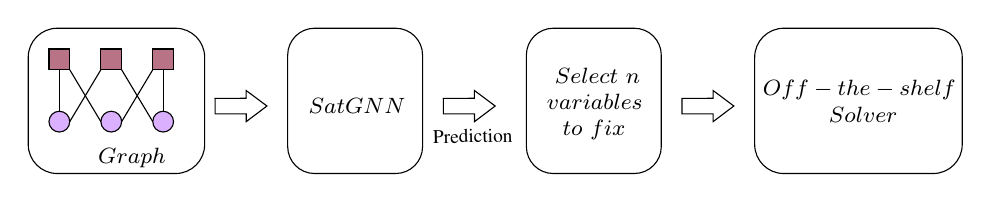
\begin{tikzpicture}[x=0.75pt,y=0.75pt,yscale=-1,xscale=1]
%uncomment if require: \path (0,451); %set diagram left start at 0, and has height of 451

%Shape: Rectangle [id:dp3587479777011455] 
\draw  [fill={rgb, 255:red, 184; green, 233; blue, 134 }  ,fill opacity=1 ] (75,295) -- (85,295) -- (85,305) -- (75,305) -- cycle ;
%Shape: Circle [id:dp623010589573948] 
\draw  [fill={rgb, 255:red, 144; green, 19; blue, 254 }  ,fill opacity=0.32 ] (100,330) .. controls (100,327.24) and (102.24,325) .. (105,325) .. controls (107.76,325) and (110,327.24) .. (110,330) .. controls (110,332.76) and (107.76,335) .. (105,335) .. controls (102.24,335) and (100,332.76) .. (100,330) -- cycle ;
%Shape: Circle [id:dp6210319224354044] 
\draw  [fill={rgb, 255:red, 144; green, 19; blue, 254 }  ,fill opacity=0.32 ] (125,330) .. controls (125,327.24) and (127.24,325) .. (130,325) .. controls (132.76,325) and (135,327.24) .. (135,330) .. controls (135,332.76) and (132.76,335) .. (130,335) .. controls (127.24,335) and (125,332.76) .. (125,330) -- cycle ;
%Shape: Circle [id:dp9356574928412065] 
\draw  [fill={rgb, 255:red, 144; green, 19; blue, 254 }  ,fill opacity=0.32 ] (75,330) .. controls (75,327.24) and (77.24,325) .. (80,325) .. controls (82.76,325) and (85,327.24) .. (85,330) .. controls (85,332.76) and (82.76,335) .. (80,335) .. controls (77.24,335) and (75,332.76) .. (75,330) -- cycle ;
%Shape: Rectangle [id:dp3734262207947956] 
\draw  [fill={rgb, 255:red, 184; green, 233; blue, 134 }  ,fill opacity=1 ] (100,295) -- (110,295) -- (110,305) -- (100,305) -- cycle ;
%Shape: Rectangle [id:dp01885589435556012] 
\draw  [fill={rgb, 255:red, 184; green, 233; blue, 134 }  ,fill opacity=1 ] (125,295) -- (135,295) -- (135,305) -- (125,305) -- cycle ;
%Straight Lines [id:da4907255353964277] 
\draw    (85,305) -- (100,330) ;
%Straight Lines [id:da9596012294566421] 
\draw    (130,305) -- (130,325) ;
%Straight Lines [id:da4248647563144248] 
\draw    (110,305) -- (125,330) ;
%Straight Lines [id:da6077808155610602] 
\draw    (110,330) -- (125,305) ;
%Straight Lines [id:da7849471865454107] 
\draw    (100,305) -- (85,330) ;
%Straight Lines [id:da019130866741998265] 
\draw    (80,305) -- (80,325) ;
%Down Arrow [id:dp06778528901825087] 
\draw   (170.04,330) -- (170.02,326.25) -- (155.03,326.29) -- (155.01,318.79) -- (170,318.75) -- (169.99,315) -- (180.01,322.47) -- cycle ;
%Rounded Rect [id:dp6272397850061886] 
\draw   (65,299) .. controls (65,291.27) and (71.27,285) .. (79,285) -- (136,285) .. controls (143.73,285) and (150,291.27) .. (150,299) -- (150,341) .. controls (150,348.73) and (143.73,355) .. (136,355) -- (79,355) .. controls (71.27,355) and (65,348.73) .. (65,341) -- cycle ;
%Rounded Rect [id:dp6283367026252633] 
\draw   (190,298) .. controls (190,290.82) and (195.82,285) .. (203,285) -- (242,285) .. controls (249.18,285) and (255,290.82) .. (255,298) -- (255,342) .. controls (255,349.18) and (249.18,355) .. (242,355) -- (203,355) .. controls (195.82,355) and (190,349.18) .. (190,342) -- cycle ;
%Rounded Rect [id:dp5504011516450884] 
\draw   (305,298) .. controls (305,290.82) and (310.82,285) .. (318,285) -- (357,285) .. controls (364.18,285) and (370,290.82) .. (370,298) -- (370,342) .. controls (370,349.18) and (364.18,355) .. (357,355) -- (318,355) .. controls (310.82,355) and (305,349.18) .. (305,342) -- cycle ;
%Rounded Rect [id:dp38041408857667824] 
\draw   (415,299) .. controls (415,291.27) and (421.27,285) .. (429,285) -- (501,285) .. controls (508.73,285) and (515,291.27) .. (515,299) -- (515,341) .. controls (515,348.73) and (508.73,355) .. (501,355) -- (429,355) .. controls (421.27,355) and (415,348.73) .. (415,341) -- cycle ;
%Down Arrow [id:dp2151743401001469] 
\draw   (280.01,330) -- (279.99,326.25) -- (265,326.29) -- (264.98,318.79) -- (279.97,318.75) -- (279.96,315) -- (289.98,322.47) -- cycle ;
%Down Arrow [id:dp19599668218528143] 
\draw   (394.99,330) -- (394.98,326.25) -- (379.99,326.29) -- (379.97,318.79) -- (394.96,318.75) -- (394.95,315) -- (404.96,322.47) -- cycle ;

% Text Node
\draw (258.63,332.91) node [anchor=north west][inner sep=0.75pt]  [rotate=-358.87] [align=left] {{\fontfamily{ptm}\selectfont {\scriptsize Prediction}}};
% Text Node
\draw (195,317.4) node [anchor=north west][inner sep=0.75pt]  [font=\footnotesize]  {$~SatGNN$};
% Text Node
\draw (71,341.4) node [anchor=north west][inner sep=0.75pt]  [font=\footnotesize]  {~~~~~~~$Graph$};
% Text Node
\draw (307,301.4) node [anchor=north west][inner sep=0.75pt]  [font=\footnotesize]  {$ \begin{array}{l}
\ Select\ n\ \\
variables\ \\
\ \ to\ fix
\end{array}$};
% Text Node
\draw (411,307.4) node [anchor=north west][inner sep=0.75pt]  [font=\footnotesize]  {$ \begin{array}{c}
Off-the-shelf\ \\
Solver
\end{array}$};


\end{tikzpicture}

}
\caption{Early fixing with SatGNN.}
\label{fig:ef-satgnn}
\end{figure}

Therefore, given a set $\hat{X}$ of random candidate solutions for a given problem instance, we compute \[
\hat{x}^* = \frac{1}{|\hat{X}|}\sum_{\hat{x}\in \hat{X}} \hat{x}\odot \hat{y}(\hat{x}) + (1-\hat{x}) \odot (1 - \hat{y}(\hat{x}))
,\] where $\odot$ is the element-wise product and $\hat{y}(\hat{x})$ is the predicted optimality of candidate solution $\hat{x}\in\hat{X}$ generated using the model from the previous experiment.
In the results reported 

Furthermore, we can say that the closer a given predicted optimal variable $\hat{x}^*_i$ is to 1 (resp. 0), the more certain the model is that that variable should be fixed at 1 (resp. 0).
Therefore, we use the model's certainty to select the variables to be fixed; that is, if we want to fix 50 binary variables, we will choose the 50 variables that the model is most certain of.
We evaluate the accuracy of the SatGNN for early fixing as a function of the number of fixed variables on the two instances of the test set.
These results can be seen in figure \ref{fig:ef-acc}.
As expected, the accuracy decreases as we include variables for which the model is less certain, to the limit of 82.5\% and 87.9\% accuracy on the two instances, which is the accuracy of the predicted optimal solution over the 1745 variables.
A summary of the model's performance when fixing all variables can be seen in Table \ref{tab:exp23-test-performance}.

\begin{figure}[!htb]
    \centering
    \includegraphics[width=0.4\textwidth]{figures/acc_97_9_6.png}
    \includegraphics[width=0.4\textwidth]{figures/acc_97_9_9.png}
    \caption{Early fixing accuracy for the two instances of the ONTS problem in the test set.}
    \label{fig:ef-acc}
\end{figure}

In face of these results, we evaluate how early fixing using SatGNN impacts the optimization performance both in terms of runtime and maximum objective value.
Specifically, we solve the two instances of the ONTS problem on the test set using Gurobi under an increasing number of fixed variables.
The results can be seen in figure \ref{fig:ef-impact}.

\begin{figure}[!htb]
    \centering
    \includegraphics[width=0.4\textwidth]{figures/runtime_obj_97_9_6.png}
    \includegraphics[width=0.4\textwidth]{figures/runtime_obj_97_9_9.png}
    \caption{Optimization results of the two ONTS instances with SatGNN-based early fixing. The objective is plotted with respect to the maximum of the original problem (without any fixed variables). Accuracy is measured with respect to the optimal value of the fixed variables.}
    \label{fig:ef-impact}
\end{figure}

As expected, correctly fixing the variables positively impacts the optimization, while wrongly fixing variables may decrease the runtime but often impacts the objective negatively.
However, we see that, at the limit, a substantial runtime reduction is achieved (90\% and 28\%, for instances 6 and 9, resp.) with a negligible objective cost (1.3\% and 0.3\%, resp.).
Beyond that, fixing more than 500 variables for instance 6 and more than 200 for instance 9 deemed the problems infeasible within a 5 minutes budget.

Given that the SatGNN model could generalize the optimality classification for larger instances of the problem, we also evaluate the impact of early fixing based on our model for the same two larger instances used in the previous experiment.
The performance on the larger instances can be seen in Figure \ref{fig:exp3-larger-instances} and in Table \ref{tab:exp23-test-performance}.
Even though these instances' sizes were not seen during training (not even during validation), the model was still able to handle them and provide sensible early fixing candidates.
The performance drop is significant in terms of accuracy and optimization performance.
In most configurations, however, the model was still able to reduce the runtime with little to no objective value reduction.

\begin{figure}[!htb]
    \centering
    \includegraphics[height=0.3\textwidth]{figures/acc_97_11.png}
    \includegraphics[height=0.3\textwidth]{figures/runtime_obj_97_11.png}
    \includegraphics[height=0.3\textwidth]{figures/acc_120_9.png}
    \includegraphics[height=0.3\textwidth]{figures/runtime_obj_120_9.png}
    \caption{Performance of SatGNN on early fixing instances larger than those seen during training and validation. Instance 97\_11 has 11 jobs, 2 more than the instances previously seen. Instance 120\_9 has the same amount of jobs but schedules for 120-time steps, 23 more than in the instances previously seen.}
    \label{fig:exp3-larger-instances}
\end{figure}

%\subsection{Discussion}

 \subsection{Illustration using a motor insurance dataset}
\label{Section7}

Understanding the causal relationships between driver and vehicle characteristics is a key step in insurance analytics, as it informs both risk assessment and premium setting.
We demonstrate the advantages of CPCM using a subset of the French MTPL motor insurance dataset \citep{sarpa2025freMTPL2}, restricted to four variables:  
``ClaimNb'' records the number of claims during the policy period (integer between 1 and 16) and lending itself naturally to a Poisson model.  
``VehPower'' and ``VehAge'' are vehicles engine power and age, and ``Exposure'' is the duration that the policy was active.  
Exponential/Gamma distribution is a natural model for variables ``VehPower'', ``VehAge'', and ``Exposure'' due to their exponential-type shapes. Since the dataset contains almost a million observations, we focus on a subset of the first $n = 1000$ records; results based on different random subsamples are provided in Appendix~\ref{Appendix_Section_simulations_Pareto}.


Fitting an LINGAM/ANM to this dataset is problematic for two reasons.  
First, the discrete nature of ``ClaimNb'' violates the continuous additive noise assumption used by most ANM methods \citep{Peters_discrete}.  
Second, the other variables are skewed, non-Gaussian and heteroskedastic, making  CPCM much more natural choice.

Using the sequential family-selection approach within CPCM and the RESIT-greedy algorithm, we obtain the graph shown in Figure~\ref{Fig_motor}. In this case, family $\mathscr{S}_1$ was selected, as the resulting graph was marked as {plausible}. In contrast, applying LiNGAM or ANM-RESIT yields markedly different structures: LiNGAM suggests $\mathrm{Exposure} \rightarrow \mathrm{VehAge} \rightarrow \mathrm{VehPower}$, while ANM-RESIT recovers only $\mathrm{VehAge} \rightarrow \mathrm{VehPower}$.  

Although the ground truth for this dataset is not perfectly clear, the results provide evidence that CPCM can recover more plausible causal structures in mixed-type insurance data than existing ANM-based or linear approaches.  
By accommodating discrete outcomes, non-Gaussian noise, heteroskedasticity and heavy-tails, CPCM produces graphs that align better with domain knowledge and avoid the misspecifications that can arise in more restrictive frameworks.  
On the other hand, CPCM can be computationally demanding for larger datasets, especially when sequential family selection is combined with many candidate parent sets.  
Furthermore, as with most observational causal discovery methods, CPCM relies on the assumption of causal sufficiency, which can be restrictive in practical applications.  






\begin{figure}[h]
\centering
\begin{tikzpicture}[
    every node/.style={draw, rectangle, rounded corners, minimum width=1.7cm, minimum height=0.9cm, align=center},
    >=stealth,
    node distance=1.2cm % reduced vertical gap
]

% Nodes
\node (VehAge) {VehAge};
\node[right=of VehAge] (VehPower) {VehPower};
\node[right=of VehPower] (Exposure) {Exposure};
\node[below=0.9cm of VehPower] (ClaimNb) {ClaimNb};

% Edges
\draw[->] (VehAge) -- (VehPower);
\draw[->] (VehAge.north east) .. controls +(1.0,0.8) and +(-1.0,0.8) .. (Exposure.north west);
\draw[->] (VehPower) -- (Exposure);
\draw[->] (VehPower) -- (ClaimNb);
\draw[->] (Exposure) -- (ClaimNb);

\end{tikzpicture}
\caption{Causal graph estimated by CPCM on the French motor insurance dataset subset.}
\label{Fig_motor}
\end{figure}







\iffalse
\subsection{Illustration using income and expenditure dataset}

We explain our methodology in detail based on real-world data that describes the expenditure habits of Philippines residents. The Philippine Statistics Authority conducts a nationwide survey of Family Income and Expenditure \citep{psa_fies} every three years. 
The dataset (taken from \cite{FamilyIncomeExpenditure}) contains over 40,000 observations primarily comprising the household income and expenditures of each household. To reduce the size and add homogeneity to the data, we consider only families of size $1$ (people living alone) above the poverty line (top 90\%, with an income of at least $80,000\,\, pesos\approx 4000\,\,dollars $ per year). We end up with $n=1417$ observations. We focus on the following variables: Total income ($X_1$), Food expenditure ($X_2$), and Alcohol expenditure ($X_3$). 

These data exhibit strong heavy-tailed behavior, presenting a significant challenge for most causal discovery approaches. For instance, while $95\%$ of the population has an annual income below $400,000\,\text{pesos}$, the top $1\%$ far exceeds $1,000,000\,\text{pesos}$. This tail structure suggests the possibility of infinite variance and even an infinite expected value for all variables. Consequently, ANM and location-scale models are highly unsuitable in this context, since $f(x) = \mathbb{E}[X_i\mid X_j=x]=\infty$. In contrast, our $CPCM(F)$ method is well-suited for heavy-tailed settings when employing a heavy-tailed choice of $F$. In economics, it is common practice to model income using Pareto or Gamma distributions \citep{lawless2002statistical}.


Our objective is to identify the causal relationships among these variables. Common sense suggests that \( \text{Income} \to \text{Food} \). However, the relationships between alcohol and other variables are not trivial. In order to discovery causal relations, we apply our \( CPCM(F_1, \dots, F_k) \) methodology, following the algorithm presented in Section \ref{Section_Algorithm}. Choice \( \{F_1, \dots, F_k\} = \mathscr{S}_1 \) leads to strong rejection of all tests, making no direction plausible. This is not surprising, as the sample size is relatively large for a single parameter to sufficiently describe the complex behavior of the data. Hence, we choose \( \{F_1, \dots, F_k\} = \mathscr{S}_2 \), as defined in Section~\ref{Section_practical_choices}. 

First, we focus on the causal relationships between pairs of random variables.  Applying Algorithm~\ref{Algorithm1} to determine the causal relationship between \( X_1 \) and \( X_2 \) yields p-values of 0.2 and 0.02 for the directions \( X_1 \to X_2 \) and \( X_2 \to X_1 \), respectively. This suggests rejecting the plausibility of the latter graph while not rejecting the former, leading to the final estimation \( X_1 \to X_2 \). Using a similar approach, we conclude that \( X_3 \to X_2 \), with p-values of \( 2 \times 10^{-9} \) and 0.16. This result suggests that drinking habits influence food habits. Finally, the p-values corresponding to \( X_1 \to X_3 \) and \( X_3 \to X_1 \) were \( 10^{-9} \) and 0.02, respectively. This indicates that some assumptions remain unfulfilled. In this case, we believe that causal sufficiency is violated due to a strong unobserved common cause between these variables. Note that even though both causal graphs were implausible, the direction \( X_3 \to X_1 \) appeared to be more probable (\(0.02 > 10^{-9} \)).

Finally, we apply the multivariate score-based algorithm presented in Section \ref{Section_score_based_algorithm} using the choice \( \{F_1, \dots, F_k\} = \mathscr{S}_2 \). The graph with the best score is \( \text{Alcohol} \to \text{Food} \leftarrow \text{Income} \). However, this graph is not plausible, as the test of independence between \( \hat{\varepsilon}_1, \hat{\varepsilon}_2, \hat{\varepsilon}_3 \) yields a p-value of 0.03. This suggests that some assumptions, such as causal sufficiency, may still be violated. 

\fi
 \section{Conclusion}
\label{sec:conclusion}

We consider top-down attention by explaining from an Analysis-by-Synthesis (AbS) view of vision. Starting from previous work on the functional equivalence between visual attention and sparse reconstruction, we show that AbS optimizes a similar sparse reconstruction objective but modulates it with a goal-directed top-down modulation, thus simulating top-down attention. We propose \model, a top-down modulated ViT model that variationally approximates AbS. We show that \model achieves controllable top-down attention and improves over baselines on V\&L tasks as well as image classification and robustness.
\clearpage
% ---- Bibliography ----
%
% BibTeX users should specify bibliography style 'splncs04'.
% References will then be sorted and formatted in the correct style.
%
\section*{Acknowledgements}
This work was supported in part by NSERC. We thank all anonymous reviewers and area chairs for their valuable comments, Hanxiao Jiang, Hang Zhou for insightful discussion, and Mingrui Zhao for help with data annotation.
\bibliographystyle{splncs04}
\bibliography{main}
\end{document}
